\documentclass[12pt,reqno]{article}
\usepackage{amsmath,amssymb,amsfonts}
\usepackage{amsthm}
\usepackage{natbib}
\usepackage{graphicx}
\usepackage{url}
\usepackage{tikz}
\usetikzlibrary{decorations.pathreplacing}
\usepackage{float}
\usepackage{booktabs,tabularx}
\usepackage{hyperref} % Added for better navigation and citation linking
\usepackage{geometry} % For flexible page layout

% Set page geometry
\geometry{a4paper, margin=1in}

\mathsurround=3pt
\allowdisplaybreaks
\newcommand{\ra}[1]{\renewcommand{\arraystretch}{#1}}

\numberwithin{equation}{section}

\makeatletter
\renewcommand{\section}{\@startsection{section}{1}{0pt}{20pt}{6pt}{\large\bf}}
\renewcommand{\@seccntformat}[1]{\csname the#1\endcsname.\ }
\makeatother

%%%%%%%%%%%%%%%%%%%%%%%%%%%%%%%%%%%%%%%%%%%%%%%%%%%%%%%%%%%%%%%%%%%%%%%%%%%%%%%
%%% Definitions - Standardized Mathematical Notation %%%
%%%%%%%%%%%%%%%%%%%%%%%%%%%%%%%%%%%%%%%%%%%%%%%%%%%%%%%%%%%%%%%%%%%%%%%%%%%%%%%

\def\EE{\mathbb{E}} % Expectation
\def\PP{\mathbb{P}} % Physical measure
\def\QQ{\mathbb{Q}} % Risk-neutral measure
\def\R{\mathbb{R}}  % Real numbers
\def\C{\mathbb{C}}  % Complex numbers
\def\cF{{\cal F}}   % Filtration
\def\cD{{\cal D}}

\def\wt{\widetilde}
\def\wh{\widehat}
\def\e{\text{e}}

\newcommand{\eps}{\varepsilon}

% Theorem environments
\newtheorem{theorem}{Theorem}[section]
\newtheorem{lemma}[theorem]{Lemma}
\newtheorem{coroll}[theorem]{Corollary}
\newtheorem{prop}[theorem]{Proposition}
\newtheorem{example}[theorem]{Example}
\theoremstyle{definition} % Set style for definitions and remarks
\newtheorem{definition}[theorem]{Definition}
\newtheorem{remark}[theorem]{Remark}
\newtheorem{ass}[theorem]{Assumption}

%%%%%%%%%%%%%%%%%%%%%%%%%%%%%%%%%%%%%%%%%%%%%%%%%%%%%%%%%%%%%%%%%%%%%%%%%%%%%%%
%%% Title & Author(s) %%%
%%%%%%%%%%%%%%%%%%%%%%%%%%%%%%%%%%%%%%%%%%%%%%%%%%%%%%%%%%%%%%%%%%%%%%%%%%%%%%%
\title{\textbf{Optimal Investment in Bitcoin Mining Farms: A Hedged Monte-Carlo Approach}}
\author{
    Y. Kitapbayev\thanks{Affiliation and contact details.} \and
    F. Macias\thanks{Affiliation.} \and
    A. Alqubaisi\thanks{Affiliation.} \and
    M. Lopez de Prado\thanks{Affiliation.} \and
    A. Lipton\thanks{Affiliation.} \and
    J.P. Zubelli\thanks{Affiliation.}
}
\date{\today}

\begin{document}

\maketitle

\begin{abstract}
The decision to invest in a Bitcoin mining facility involves navigating significant uncertainties, primarily driven by the high volatility of Bitcoin prices and fluctuating energy costs. This paper analyzes the optimal timing for such investments within a real options framework. We formulate the investment as an optimal stopping problem, considering both the option to defer the investment and the operational flexibility to temporarily suspend mining activities when unprofitable. To solve this complex valuation problem, we employ the Hedged Monte Carlo (HMC) method. HMC enhances the accuracy of the estimate by incorporating hedge sensitivities (Greeks) as control variables, thus reducing the variance of the Monte Carlo estimator. This approach allows for robust valuation under the real-world probability measure, accommodating complex dynamics for the underlying stochastic factors. We present a framework for determining the strategic value and optimal investment threshold for large-scale cryptocurrency mining projects \\.\\


{\bf HIGHLIGHTS}
\begin{itemize}
    \item Motivation: Evergroing Bitcoin cost due to energy consumption 
    \item Determination of a suitable basis to tackle this problem (namely Margrabe type)
    \item Sustainability issues and energy consumptions
    \item Innovative usage of Real Options in the context of bit coin farming decisions
    \item Usage of the bitcoin index as a proxy to the actual bitcoin price. 
\end{itemize}

IMPORTANT TOOL THE HASHPRICE \url{https://data.hashrateindex.com/network-data/bitcoin-hashprice-index}

\end{abstract}

\textbf{Keywords:} Real Options, Bitcoin Mining, Optimal Stopping, Hedged Monte Carlo, Investment under Uncertainty, Energy Finance.

\section{Introduction}

The global expansion of Bitcoin mining operations represents a significant industrial development, characterized by substantial capital expenditures and high energy consumption. The economic viability of these ventures is inherently uncertain, being highly sensitive to the volatile market price of Bitcoin (BTC) and the cost of electricity. The scale of these investments is notable; for example, the establishment of a \$ 2 billion crypto mining facility on Reem Island by the Phoenix group and the Abu Dhabi government underscores the strategic importance of robust valuation methods in this sector.

Given the irreversibility of the initial investment and the high uncertainty of future cash flows, traditional discounted cash flow (DCF) analysis is inadequate, as it fails to capture the value of managerial flexibility. Real Options Analysis (ROA) provides a superior framework, recognizing that investors possess critical flexibilities: the option to defer the investment (timing flexibility) and the option to suspend operations if the mining margin becomes negative (operational flexibility).

The main goal of this paper is to analyze the strategic value of investing in a Bitcoin mining farm under uncertainty. We model this decision as an optimal stopping problem with the objective of maximizing the expected net present value (NPV) by choosing the optimal time to execute the project.

Valuing these combined options (timing and switching) in the presence of multiple stochastic factors presents computational challenges. While traditional methods like binomial trees or finite difference methods exist, they often become intractable in higher dimensions or with complex dynamics. Monte Carlo simulation methods, particularly the Least-Squares Monte Carlo (LSM) approach \cite{LongstaffSchwartz2001}, are frequently used, but can suffer from estimation biases and inefficiency.

To address these challenges, we utilize the Hedged Monte Carlo (HMC) method \cite{Bouchaud, JPZ}. HMC is a variance reduction technique that leverages information about the sensitivities (deltas) of the option value to the underlying assets. By incorporating the hedging strategy directly into the simulation as a control variate, HMC provides a more stable and accurate estimation of the continuation value and the optimal exercise boundary. Furthermore, HMC can be easily applied under the real-world probability measure $\PP$, using a subjective discount rate, which avoids the complexities of estimating the market price of risk for non-tradable assets.

This paper contributes to the literature by applying the HMC methodology to the specific context of Bitcoin mining investment decisions, offering a robust and flexible tool for strategic planning in this emerging industry.

\section{Literature Review}

\paragraph{Fast mean-reverting stochastic volatility.}
Asymptotic analysis of invest-or-wait problems under fast mean-reverting stochastic volatility shows that stochastic volatility raises the value of waiting and shifts the optimal investment boundary relative to constant-volatility benchmarks \citep{SouzaZubelli2011ASMBI}.

\paragraph{Mean-reverting project value and investment cost.}
When both the project value and the investment cost are mean-reverting, the optimal trigger becomes genuinely two-dimensional; simple value-to-cost ratio rules hold only in special cases, and the problem is addressed numerically \citep{JaimungalSouzaZubelli2013EJF}.

\paragraph{Hedged Monte Carlo in incomplete markets.}
For settings driven by historical/simulation scenarios—common in commodities—Zubelli and coauthors propose a hedged Monte Carlo approach that prices the real option jointly with a dynamically learned hedge \citep{BrigattiMaciasSouzaZubelli2015FIC}.

\paragraph{Energy application: LNG contracts.}
These ideas extend to energy, where robust, risk-aware valuation and management of LNG contracts with cancellation options are formulated and solved within an optimization framework \citep{GuiguesSagastizabalZubelli2014JOTA}.

% [Placeholder: This section should be added by the authors. It should cover:]
% 1. The economics and drivers of Bitcoin mining profitability (hash rate, difficulty, energy costs).
% 2. Applications of Real Options Analysis in mining and energy investments, especially those involving switching/mothballing options.
% 3. Overview of numerical methods for optimal stopping problems, comparing LSM and HMC, highlighting the advantages of variance reduction techniques.

\section{Problem Formulation}

We formalize the investment decision faced by a company considering the establishment of a Bitcoin mining farm.

\subsection{Investment Setup}

Consider an investment horizon $[0,T]$. The company has the option to build a mining farm, requiring a fixed, irreversible sunk cost $K>0$. If the company invests at time $\tau \in [0,T]$, the farm begins operations immediately and has a fixed operational lifetime $T'$. Consequently, the farm operates during the interval $[\tau, \tau+T']$.

\begin{figure}[H]
    \centering
    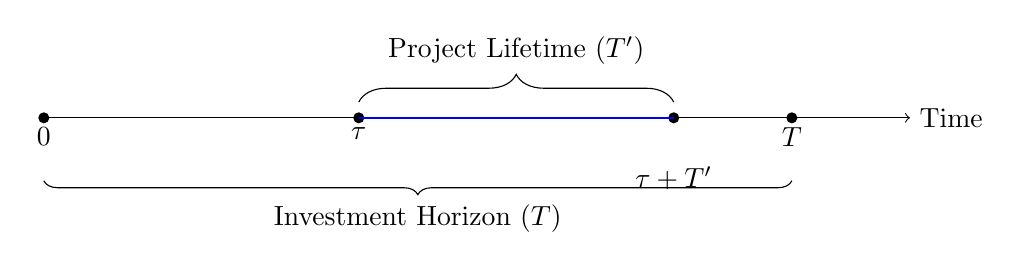
\begin{tikzpicture}
        % Draw the main timeline
        \draw[->] (0,0) -- (11,0) node[right] {Time};

        % Draw the points
        \fill (0,0) circle (2pt) node[below] {$0$};
        \fill (4,0) circle (2pt) node[below] {$\tau$};
        \fill (9.5,0) circle (2pt) node[below] {$T$};
        \fill (8,0) circle (2pt); % T'+tau

         \node[below] at (8,-0.5) {$\tau+T'$};

        % Highlight the operational period
        \draw[thick, blue] (4,0) -- (8,0);

        % Brace above the operational period
        \draw [decorate,decoration={brace,amplitude=10pt}] (4,0.2) -- (8,0.2) node[midway, above=10pt] {Project Lifetime ($T'$)};
         % Brace below the investment horizon
        \draw [decorate,decoration={brace,amplitude=5pt,mirror}] (0,-0.8) -- (9.5,-0.8) node[midway, below=5pt] {Investment Horizon ($T$)};

    \end{tikzpicture}
    \caption{Timeline of the investment decision and project operation.}
    \label{fig:timeline}
\end{figure}

\subsection{Stochastic Variables and Cash Flows}

The profitability of the mining farm is driven by two primary stochastic processes:
\begin{itemize}
    \item $X_t$: The price of 1 BTC in USD at time $t$.
    \item $Y_t$: The electricity price in USD/MWh at time $t$.
\end{itemize}
We assume the dynamics of $X_t$ and $Y_t$ are known or simulated under the real-world measure $\PP$. Valuation is performed using a discount rate $\rho$, reflecting the company's cost of capital (WACC).

\subsubsection{Net Present Value (NPV) of the Project}

If the investment is made at time $\tau$, the Net Present Value (NPV) of the project, evaluated at time $\tau$, is given by:
\begin{align}
    G(x,y) = \EE_{x,y}^{\PP}\left[\int_\tau^{\tau+T'}e^{-\rho(t-\tau)}\left( (X_t-\kappa Y_t)^+ - k\right)dt\right] - K
\end{align}
where $\EE_{x,y}^{\PP}[\cdot]$ denotes the expectation under $\PP$ conditional on $X_\tau=x$ and $Y_\tau=y$. The parameters are:
\begin{itemize}
    \item $\kappa$: The electricity consumption factor (MWh required to mine 1 BTC per unit time), capturing hardware efficiency and network difficulty.
    \item $k$: Fixed operating costs per unit time (e.g., maintenance, wages).
    \item $K$: The initial sunk cost.
\end{itemize}

We assume the firm has the operational flexibility to suspend mining (switch to an idle state) and resume operations without cost. The optimal strategy is to mine if $X_t > \kappa Y_t$, and stay idle otherwise. The instantaneous variable cash flow is thus $(X_t-\kappa Y_t)^+ := \max(X_t-\kappa Y_t, 0)$. The fixed cost $k$ is incurred regardless of the operational state.

If the processes $X_t$ and $Y_t$ are time-homogeneous, the NPV function $G$ depends only on the current values $(x,y)$.

\subsubsection{Monte Carlo Estimation of NPV}

The NPV function $G(x,y)$ must generally be estimated using Monte Carlo simulation. Discretizing the lifetime $[0,T']$ into $J$ intervals of length $h=T'/J$, the MC estimator is:
\begin{equation}
\widehat{G}(x,y) \approx \frac{h}{N}\sum_{n=1}^N \sum_{i=1}^J e^{-\rho t_i}\left( \left(X^{(n)}_{t_i}-\kappa Y^{(n)}_{t_i}\right)^+ - k\right) - K
\end{equation}
where $N$ is the number of simulated paths starting from $(x,y)$. Note that evaluating $G(x,y)$ is computationally intensive, requiring a nested simulation whenever the option value is calculated.

\section{The Hedged Monte Carlo Methodology}

The objective is to find the optimal investment time $\tau$ to maximize the expected discounted value of the project. This is formulated as an optimal stopping problem:
\begin{equation}
    V(x,y) = {\mathrm{ess}}\sup_{0\le \tau\le T} \EE_{x,y}^{\PP}\left[e^{-\rho\tau}G(X_\tau,Y_\tau)\right]
\end{equation}
where the supremum is taken over all stopping times $\tau$ adapted to the filtration generated by $(X_t, Y_t)$.

We apply the Hedged Monte Carlo (HMC) method to solve this problem. HMC utilizes dynamic programming and incorporates hedging information to improve the estimation of the continuation value.

\subsection{Discretization and Backward Induction}

We discretize the investment horizon $[0,T]$ into $L$ intervals of length $\Delta=T/L$, with time points $t_j=j \Delta$. We simulate $M$ independent trajectories of $(X, Y)$ over this grid.

The algorithm proceeds via backward induction. At the terminal time $T=t_L$, the value is:
\begin{equation}
    V(L,m) = G(X^{(m)}_T, Y^{(m)}_{T})
\end{equation}
for the $m$-th simulated path.

At time step $t_j$, the company compares the immediate investment value, $G(X_{t_j}, Y_{t_j})$, with the continuation value, $CV(j, X_{t_j}, Y_{t_j})$. We approximate the continuation value using a regression on a set of basis functions $\{C_a(x,y)\}_{a=1}^B$:
\begin{equation}
    CV(j,x,y) \approx \sum_{a=1}^B \gamma_a^j C_a(x,y)
\end{equation}

\subsection{HMC Regression}

In the HMC approach, the coefficients $(\gamma_a^j)$ and the hedging coefficients $(\beta_a^j, \delta_a^j)$ are determined simultaneously by minimizing the squared replication error of the hedged portfolio. This minimization leverages the fact that the discounted option price process, when appropriately hedged, behaves like a martingale.

The objective function to minimize is:
\begin{align}
\min_{\gamma, \beta, \delta} \sum_{m=1}^{M}\Bigg( &e^{-\rho \Delta} V\left(j+1, X_{t_{j+1}}^{(m)}, Y_{t_{j+1}}^{(m)}\right) - \sum_{a=1}^B \gamma_a^j C_a\left(X_{t_j}^{(m)}, Y_{t_j}^{(m)}\right) \nonumber \\
& + \sum_{a=1}^B \beta_a^j \frac{\partial C_a}{\partial x}\left(X_{t_j}^{(m)}, Y_{t_j}^{(m)}\right)\left[X_{t_j}^{(m)} - e^{-\rho\Delta} X_{t_{j+1}}^{(m)}\right] \nonumber \\
& + \sum_{a=1}^B \delta_a^j \frac{\partial C_a}{\partial y}\left(X_{t_j}^{(m)}, Y_{t_j}^{(m)}\right)\left[Y_{t_j}^{(m)} - e^{-\rho\Delta} Y_{t_{j+1}}^{(m)}\right]
\Bigg)^2
\end{align}

The terms involving $\beta_a^j$ (hedging $X$) and $\delta_a^j$ (hedging $Y$) act as control variates. They represent the P\&L of delta-hedge portfolios constructed using the known sensitivities of the basis functions. By incorporating these "perfect hedges" for the basis functions, HMC significantly reduces the variance in the estimation of the continuation value.

\subsection{Option Value Update}

Once the coefficients $\hat{\gamma}_a^j$ are estimated, the continuation value is calculated. The project value at time $t_j$ for path $m$ is then:
\begin{equation}
    V(j,m) = \max\left( G(X_{t_j}^{(m)},Y_{t_j}^{(m)}), \sum_{a=1}^B \hat{\gamma}_a^j C_a\left(X_{t_j}^{(m)},Y_{t_j}^{(m)}\right) \right)
\end{equation}
This process is repeated backwards until $t_0$, yielding the value of the investment option.

\section{Numerical Implementation and Case Study}


% [Placeholder: This section is crucial and must be developed by the authors.]

% \subsection{Stochastic Models and Calibration}
% [Specify the SDEs used for X_t (BTC) and Y_t (Electricity). Justify the choice of models (e.g., GBM, Mean-Reversion, Jumps) and describe the calibration process using historical data.]

% \subsection{Case Study Parameters}
% [Define the base case parameters: K (Sunk Cost), T (Horizon), T' (Lifetime), kappa (Efficiency), k (Fixed Costs), rho (WACC).]

% \subsection{HMC Implementation Details}
% [Specify the numerical parameters: L, J (Time steps); M, N (Simulation counts). Crucially, detail the choice of basis functions C_a(x,y) (e.g., Polynomials, Laguerre).]

We assume that we will build a farm with 1,000 TH capacity. Suppose we install Bitcoin miner S12 pro machines, each of which has 234 TH at a price \$3,744, i.e., approximately four machines are required. Each machine operates with a nominal power of  3.51 KW. The electricity price $Y$ is in \$/KWh. Total energy per year required is $\kappa= \frac{1000}{234}\times3.51\times 24\times 365$ KWh. The energy cost per year is $\int_0^1 \kappa Y_t dt$.  Assuming the fixed electricity rate $Y_0= 0.05$ \$/KWh, it will be \$ 6,570. The investment cost for machines is  $K_1=\frac{1000}{234}\times 3,744$ \$, the infrastructure cost (cables, labor) $K_2=0.06\times K_1$ \$, the cost of containers $K_3=\frac{1000}{234}\times 100,000/210$ \$, $K_4$ is the cost of the rental of land. The total investment cost is $K=K_1+K_2+K_3+K_4$. The lifetime period of machines is  $T'= 3-4$ years.

We work with the hashprice index $X$. Current value (as of 23 May 2025) is \$50 per 1 PH (or 1,000 TH) per day. Hence, if $X$ stays the same at this level, the annual revenue is $50\times 365=18,250$ \$.

\section{Results and Discussion}
% [Placeholder: This section must present the findings.]

% \subsection{Optimal Investment Boundary}
% [Present the estimated option value V_0. Visualize the Optimal Investment Boundary in the (X, Y) space, which separates the "Wait" and "Invest" regions.]

% \subsection{Sensitivity Analysis}
% [Analyze the impact of key parameters (e.g., volatility of X and Y, correlation, discount rate rho) on the option value and the investment boundary.]

% \subsection{Comparison with LSM}
% [To validate the HMC approach, compare the results (accuracy, variance, computational time) with the standard Least-Squares Monte Carlo (LSM) method.]

\section{Conclusion}

This paper presents a framework for valuing investments in Bitcoin mining facilities using real options analysis. By employing the Hedged Monte Carlo method, we address the complexities arising from stochastic Bitcoin prices and electricity costs, the option to defer investment, and the operational flexibility inherent in mining operations. The HMC approach provides a robust and variance-reduced method for determining the optimal investment timing under uncertainty.

% [Summarize the main findings from the results section and discuss future research directions.]

\appendix
\section{Appendix: Overview of Bitcoin Mining}

% [This appendix has been revised for a professional tone. The original note regarding ChatGPT has been removed, assuming the content is verified by the authors.]

Bitcoin mining is the decentralized consensus mechanism by which transactions are validated and added to the blockchain, and new bitcoins are issued. It relies on the \textbf{Proof-of-Work (PoW)} protocol, requiring participants (miners) to expend significant computational effort to solve complex cryptographic puzzles \cite{narayanan2016bitcoin}.

\subsection{Process and Rewards}
Miners aggregate transactions into a candidate block and repeatedly hash the block header until they find a value below a network-defined target (the difficulty). This requires specialized hardware, predominantly \textbf{Application-Specific Integrated Circuits (ASICs)}.

The successful miner broadcasts the block, and upon validation by the network, receives a block reward. This reward consists of the block subsidy (newly minted bitcoins) and transaction fees \cite{nakamoto2008bitcoin, antonopoulos2017mastering}. The network difficulty adjusts approximately every two weeks to maintain an average block discovery time of ten minutes. The block subsidy halves roughly every four years; as of the 2024 halving, the subsidy is 3.125 BTC.

\subsection{Mining Strategies and Time to Reward}

The time until a mining farm generates revenue depends on its strategy:

\begin{itemize}
    \item \textbf{Pool Mining:} Miners combine their hash rate in a pool and share rewards proportionally. This reduces the variance of returns, allowing for consistent, frequent payouts (hours or days).
    \item \textbf{Solo Mining:} The farm keeps the entire block reward if it successfully mines a block. However, the time to discover a block is stochastic and can be extremely long, following an exponential distribution.
\end{itemize}

\subsection{Illustrative Numerical Example}

This example calculates the expected revenue for a hypothetical mining farm.

\paragraph{Assumptions (Illustrative):}
% [Generalized the assumptions rather than relying on a specific future date.]
\begin{itemize}
    \item Global Network Hash Rate ($H_{Global}$): $965~\mathrm{EH/s}$ (1 EH/s = $10^{18}$ H/s).
    \item Block Reward ($R$): $3.125~\mathrm{BTC}$.
    \item Average Blocks per Day ($B_{Day}$): $144$.
    \item Farm Hash Rate ($H_{Farm}$): $20~\mathrm{PH/s}$ (0.020 EH/s).
\end{itemize}

\paragraph{Calculations:}
The farm's share of the global hash rate ($\alpha$):
\[
\alpha = \frac{H_{Farm}}{H_{Global}} = \frac{20~\mathrm{PH/s}}{965{,}000~\mathrm{PH/s}} \approx 2.07\times 10^{-5} \quad (0.00207\%).
\]

Expected blocks mined per day by the farm ($E[B_{Farm}]$):
\[
E[B_{Farm}] = B_{Day} \times \alpha = 144 \times 2.07\times 10^{-5} \approx 0.00298~\mathrm{blocks/day}.
\]

Expected time to mine one block (solo mining, mean of exponential distribution):
\[
\frac{1}{E[B_{Farm}]} \approx \frac{1}{0.00298} \approx 335~\text{days}.
\]

Median time-to-first block (solo mining):
\[
\frac{\ln(2)}{E[B_{Farm}]} \approx \frac{0.693}{0.00298} \approx 232~\text{days}.
\]

Expected daily revenue in BTC (assuming pool mining and ignoring fees):
\[
E[\text{Revenue}_{BTC}] = E[B_{Farm}] \times R = 0.00298 \times 3.125 \approx 0.00933~\mathrm{BTC/day}.
\]

\paragraph{Interpretation:}
For this hypothetical farm, solo mining presents high variance, with an average wait of 335 days to find a block. Pool mining provides a much more stable expected revenue stream.

\bibliographystyle{plainnat} % Recommended style for natbib
% \bibliography{bitcoin_refs,bibli}

% Placeholder References (Authors must ensure these are in their .bib files)
\begin{thebibliography}{99}

\bibitem{antonopoulos2017mastering} Antonopoulos, A. M. (2017). \textit{Mastering Bitcoin: Programming the Open Blockchain}. O'Reilly Media, Inc.

\bibitem{Bouchaud} Potters, M., Bouchaud, J.P., \& Sestovic, D. (2001). Hedged Monte Carlo: A variance reduction technique for American options. \textit{Wilmott Magazine}.

\bibitem{LongstaffSchwartz2001} Longstaff, F. A., \& Schwartz, E. S. (2001). Valuing American Options by Simulation: A Simple Least-Squares Approach. \textit{The Review of Financial Studies}, 14(1), 113-147.

\bibitem{nakamoto2008bitcoin} Nakamoto, S. (2008). Bitcoin: A Peer-to-Peer Electronic Cash System.

\bibitem{narayanan2016bitcoin} Narayanan, A., et al. (2016). \textit{Bitcoin and Cryptocurrency Technologies: A Comprehensive Introduction}. Princeton University Press.

\bibitem{JPZ} [Reference related to J.P. Zubelli's work on HMC if applicable].

\end{thebibliography}

\end{document}